\documentclass[10pt]{article}
\usepackage{mathpaper}

\begin{document}
\papertitle{试卷标题}
\paperinformation{时间:2小时 \ \ \ \ 满分:120分}
\begin{questions}{\selectingintroduction}
    \question %1
    \question %2
    \question %3
    \question %4
    \question %5
    \question %6
    \question %7
    \question %8
    \question %9
    \question 如图,在平行四边形$ABCD$中,$BC=2AB=20$,$B$、$F$、$E$三点共线,且$\angle ABC=60^{\circ}$。连$AF$、$AE$、$CE$,若$AE=EF$,$\angle DAE+\angle CBF=60^{\circ}$,且$AF=6$,则$\Delta BEC$的面积为(~~~~~~~)。
    \onp{$16\sqrt{3}$}{$68\sqrt{3}$}{$32\sqrt{3}$}{$34\sqrt{3}$}
    \begin{figure}[htb]
        \centering
        \subfigure[(第10题)]{
        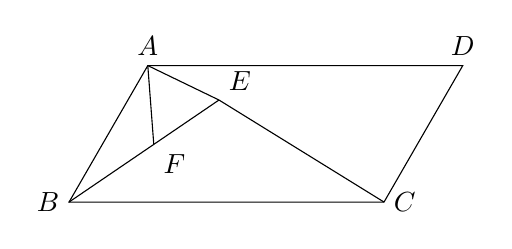
\begin{tikzpicture}[scale=0.4]
            \coordinate[label=above:{$A$}] (A) at (2.5,4.33333);
            \coordinate[label=left:{$B$}] (B) at (0,0);
            \coordinate[label=above:{$D$}] (D) at (12.5,4.33333);
            \coordinate[label=right:{$C$}] (C) at (10,0);
            \coordinate[label=above right:{$E$}] (E) at (4.76,3.24);
            \coordinate[label=below right:{$F$}] (F) at (2.69,1.83);
            \draw (A)--(B)--(C)--(D)--cycle;
            \draw (A)--(F);
            \draw (A)--(E);
            \draw (C)--(E);
            \draw (B)--(E);
        \end{tikzpicture}}
    \end{figure}
\end{questions}
\begin{questions}{\complitingintroduction}
    \question %11
    \question %12
    \question %13
    \question %14
    \question %15
    \question %16
\end{questions}
\begin{questions}{\answeringintroduction}
    \question %17
    \begin{subquestions}
        \subquestion %17.1
        \subquestion %17.2
    \end{subquestions}
    \question %18
    \begin{subquestions}
        \subquestion %18.1
        \subquestion %18.2
    \end{subquestions}
    \question %19
    \begin{subquestions}
        \subquestion %19.1
        \subquestion %19.2
    \end{subquestions}
    \question
    \begin{subquestions}
        \subquestion %20.1
        \subquestion %20.2
    \end{subquestions}
    \question %21
    \begin{subquestions}
        \subquestion %21.1
        \subquestion %21.2
    \end{subquestions}
    \question %22
    \begin{subquestions}
        \subquestion %22.1
        \subquestion %22.2
        \subquestion %22.3
    \end{subquestions}
    \question %23
    \begin{subquestions}
        \subquestion %23.1
        \subquestion %23.2
        \subquestion %23.3
    \end{subquestions}
    \question %24
    \begin{subquestions}
        \subquestion %24.1
        \subquestion %24.2
        \subquestion %24.3
    \end{subquestions}
\end{questions}
\end{document}